\chapter{Анализ проблематики задач классификации когнитивных состояний}
\label{chapter1}
\begin{annotation}
	В этом разделе описаны алгоритмы решения типовых задач классификации, кластеризации, \ldots
\end{annotation}

Это обзорно-аналитическая глава, в которой требуется отразить:

\begin{itemize}
	\item результат изучения различных существующих методов решения задач в рамках проблематики УИРа/диплома (иногда даже в смежных областях), это обзорный аспект, который пишется, в основном, на основе имеющейся литературы или/и программного обеспечения;
	\item сравнение (с какой-либо определенной целью) этих методов и средств.
\end{itemize}

Приведенные ниже названия пунктов являются очень примерными, их состав и структура сильно зависят от специфики конкретной работы.




%Большие отсупы --- это хорошо. Облегчает чтение длинных <<простыней>> текста
\section{Изучение и анализ подходов к классификации когнитивных состояний по данным фМРТ (статическим и динамическим) применительно к задачам медицинской диагностики \dots}

\begin{annotation}
В случае РСПЗ, так оформляется аннотация к разделу. Такая же аннотация, только более общая, должна быть для главы. После аннотации может следовать рабочая или финальная версия текста соответствующего раздела. В случае ПЗ, таких аннотаций быть не должно.
\end{annotation}

\dots

Результаты анализа полезно оформлять в виде таблиц (см. табл. \ref{tbl:cmp-1}).

\begin{table}%
\caption{Результаты сравнения нескольких программных систем}\label{tbl:cmp-1}
\centering
\begin{tabular}{|l|l|c|c|c|c|}

\hline

\textnumero & Название системы & Показатель 1 & Показатель 2 & Показатель 3 & Показатель 4 \\

\hline

\end{tabular}
\end{table}

Сначала приведем пример более сложной таблицы (см. табл. \ref{tbl:cmp-adv} и 
\ref{tbl:cmp-2}).

\begin{table}%
\caption{Таблица с длинным, многострочным названием, чтобы показать, как форматируется такой заголовок}
\label{tbl:cmp-adv}
\centering
\begin{tabular}{|l|l|c|c|c|c|}

\hline

\textnumero & Название системы & Показатель 1 & Показатель 2 & Показатель 3 & Показатель 4 \\

\hline

\end{tabular}
\label{tbl:cmp-2}
\end{table}


А теперь, продемонстрируем, как должна выглядеть иллюстрация (см. рис. \ref{pic:lambda-cube}).

\begin{figure}%
\begin{center}
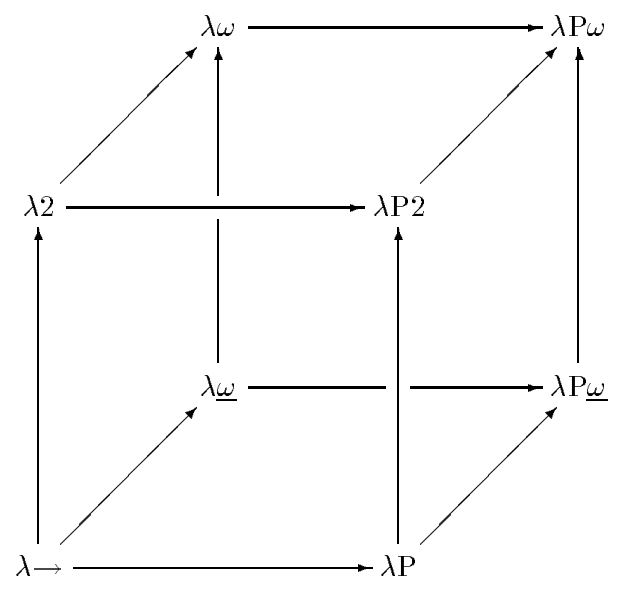
\includegraphics[width=.5\columnwidth]{./img/lambda-cube.png}%
\end{center}
\caption{Ламбда-куб Барендрегта}%
\label{pic:lambda-cube}%
\end{figure}

\dots





\section{Сравнительный анализ методов классификации многомерных данных (линейный дискриминантный анализ, метод опорных векторов, нейросетевые методы) для выбора  подходящего набора алгоритмов. \dots}

\dots





\section{Сравнительный анализ программных средств визуализации трехмерных данных фМРТ и исследование возможности их использования.}

\begin{figure}%
	\begin{center}
		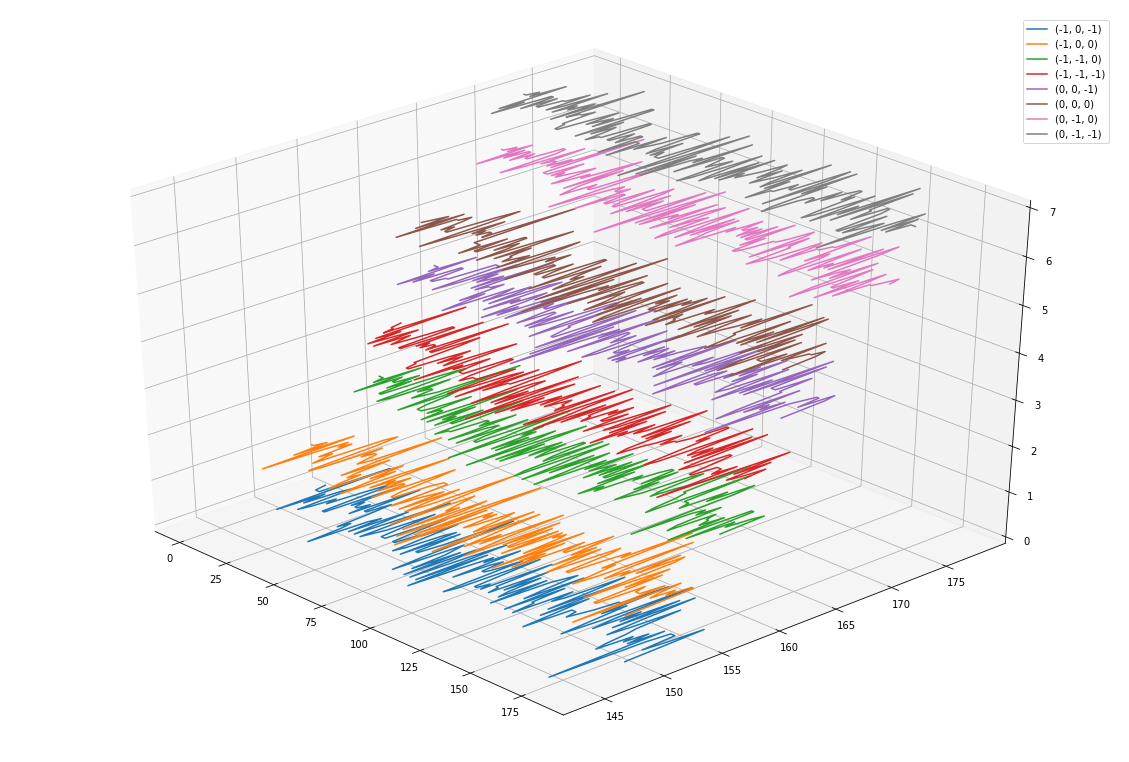
\includegraphics[width=.7\columnwidth]{./img/local_100c.png}%
	\end{center}
	\caption{Пример активности локальной окрестности вокселя в течение \~47 сек}%
	\label{pic:local_100c}%
\end{figure}




\section{Выводы и постановка задачи курсового проекта}

Это всегда последний пункт. Здесь, по-первых, приводятся, попунктно, основные вывода из проделанного анализа. Например:

\begin{enumerate}
	\item Выполнен сравнительный анализ таких-то формальных систем с точки зрения применимости к решению такой-то задачи. Ни одна из проанализированных напрямую не подходит, поэтому требуется разработать вариацию на основе системы такой-то.
	\item Были проанализированы варианты программных архитектур на основе систем. С учетом требований к поддержке больших объемов данных и высоких требований к потенциалу модернизируемости, была выбрана за основу такая-то архитектура.
	\item Сравнительный анализ таких-то библиотек показал, что библиотека X проще в использовании, но менее производительна, в то время как библиотека Y обеспечивает высокую производительность, но и требует значительных трудозатрат для использования. В связи с такими-то соображениями были принято решение использовать такую-то библиотеку.
\end{enumerate}

Далее пишется постановка задачи, на основе выданного задания. Это должен быть связный текст в объеме до 1-1,5 страниц. В этом разделе необходимо раскрыть цели и задачи УИРа/диплома.